\documentclass[xcolor=dvipsnames]{beamer}
% \documentclass[handout]{beamer} % This version collapses all overlays
% \usepackage{pgfpages}
% \mode<handout>{\setbeamercolor{background canvas}{bg=black!3}}
% \pgfpagesuselayout{4 on 1}[letterpaper,border shrink=5mm, landscape]
% % \pgfpagesuselayout{8 on 1}[letterpaper,border shrink=5mm]
%% This is the file main.tex

\frenchspacing
% \beamertemplatenavigationsymbolsempty
\newcommand{\E}{\mbox{E}}
\newcommand{\Var}{\mbox{Var}}
\newcommand{\z}[1]{{\color{RedOrange}#1}}
% \newcommand{\newblock}{}

\usetheme{Singapore}
% \usetheme{Montpellier}
% \usetheme{Berlin}
% \usetheme{Malmoe}

\mode<presentation>
{
  % \usetheme{Warsaw}
  % or ...

  % \setbeamercovered{transparent}
  % or whatever (possibly just delete it)
}

\usepackage{natbib}
\usepackage[english]{babel}
% \usepackage[latin1]{inputenc}
% \usepackage{times}
\usepackage[T1]{fontenc}
% Or whatever. Note that the encoding and the font should match. If T1
% does not look nice, try deleting the line with the fontenc.


\title[]
{Reproducing Shakespeare}
\subtitle
{In honor of Bradley Efron's 80th birthday}

\author{Ronald A. Thisted}
% \author{R. A. Thisted}
% - Use the \inst{?} command only if the authors have different
%   affiliation.

\institute[The University of Chicago] % (optional, but mostly needed)
{
  Departments of Statistics and Public Health Sciences\\
  The University of Chicago
}
% - Use the \inst command only if there are several affiliations.
% - Keep it simple, no one is interested in your street address.

\date
{24 May 2018}

\subject{Talks}
% This is only inserted into the PDF information catalog. Can be left out. 
% Delete this, if you do not want the table of contents to pop up at
% the beginning of each subsection:
\AtBeginSection[]
{
  \begin{frame}<beamer>
    \frametitle{GPS}
    \tableofcontents[currentsection]
  \end{frame}
}


% If you wish to uncover everything in a step-wise fashion, uncomment
% the following command: 

%\beamerdefaultoverlayspecification{<+->}

\begin{document}

\begin{frame}
  \titlepage
\end{frame}
	\begin{frame}
    \frametitle{Estimating Shakespeare's vocabulary}
    \begin{center}
        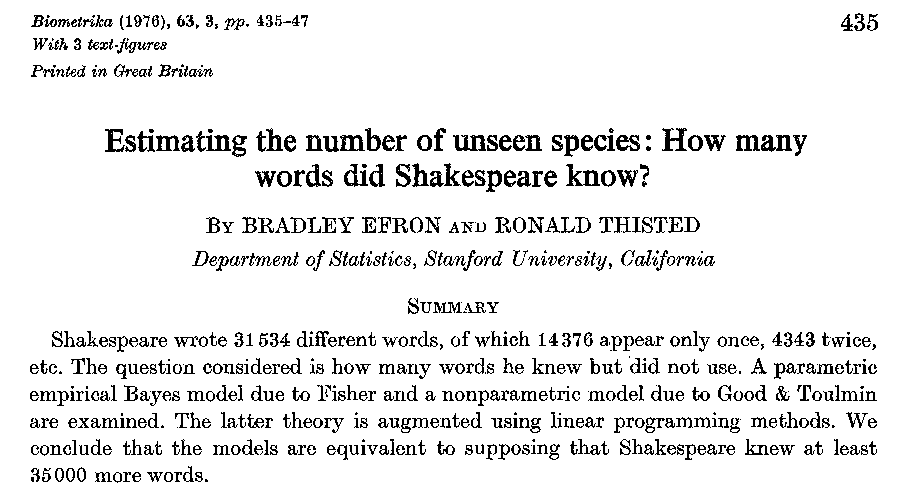
\includegraphics[width=4in]{../compendium/Figures/ET-Titles.pdf}        
    \end{center}
		\pause
	
	{\color{red}Are these results reproducible?}
\end{frame}


% \section{Outline}
\begin{frame}
  \frametitle{Roadmap}
  \tableofcontents
\end{frame}

\section[Repro Res]{Reproducible research}
	\begin{frame}
    \frametitle{Elements of reproducible research}
	``Reproducible Research (RR) is the practice of distributing, along with a research publication, all data, software source code, and tools required to reproduce the results discussed in the publication.'' ---James Ware (\citeyear{Ware:2010aa})
	
	\bigskip

Components of a research project compendium that affect reproducibility:
	\begin{enumerate}
		\item the underlying data,
		\item the computer programs or scripts used for calculation,
		\item the hardware and operating system under which those programs were run, and
		\item the choices of inputs to the calculations, and the process by which those choices were made.
	\end{enumerate}
\end{frame}


\section[S's vocabulary]{Estimating Shakespeare's vocabulary}
	\begin{frame}
    \frametitle{The data set from ET 1976}
    \begin{center}
        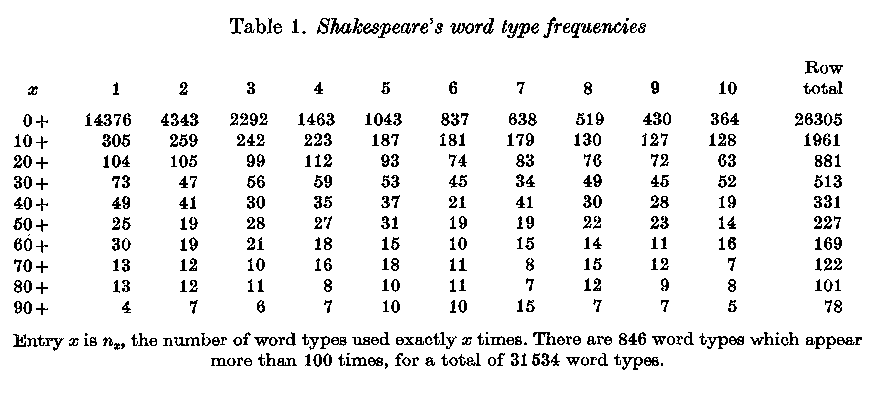
\includegraphics[width=4in]{../compendium/Figures/ET-Table1.pdf}        
    \end{center}
	
	According to Spevack's \textit{Concordance} (\citeyear{Spevack:1968qd}), the total number of words in the Shakespeare corpus was $S=884\,647$.
\end{frame}

	\input{Slides/Shakespeare-Model-Basic}
	\begin{frame}
    \frametitle{Estimates from the negative binomial model}
	With estimates for $\eta_1$, $\alpha$, and $\gamma$, we can use (\ref{eq:deltaAG}) to estimate the number of new words we would see in $tS$ ``more'' Shakespeare.
	\medskip
	
	For $\hat\eta_1$ we used the unbiased estimate $n_1$, and for $\alpha$ and $\gamma$ we used the observed data for the first $x_0$ frequency counts, $x_0=5, 10, 15, 20, 30,$ and~$40$ to calculate maximum likelihood estimates from the NB model.
	\pause
	
	Here is what we got:
	\vspace*{-5mm}
	\begin{center}
		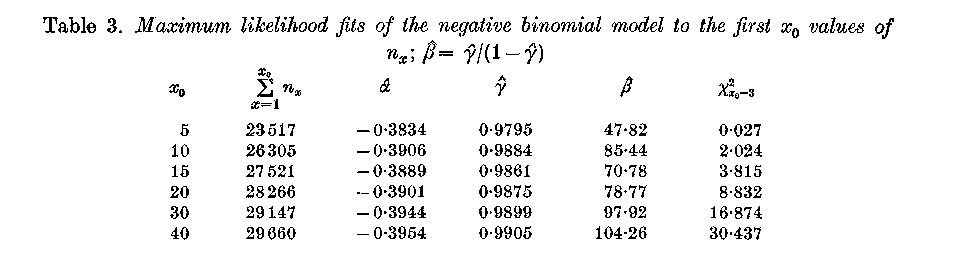
\includegraphics[width=4.5in]{../compendium/Figures/ET-Table3.pdf}
	\end{center}
	\pause	
	{\color{red} Can Table~3 be reproduced?}
\end{frame}

\section[Then]{Reproducing Results from ET 1976---Then}
	\begin{frame}
    \frametitle{The GitHub repository for ET 1976}
    \begin{center}
        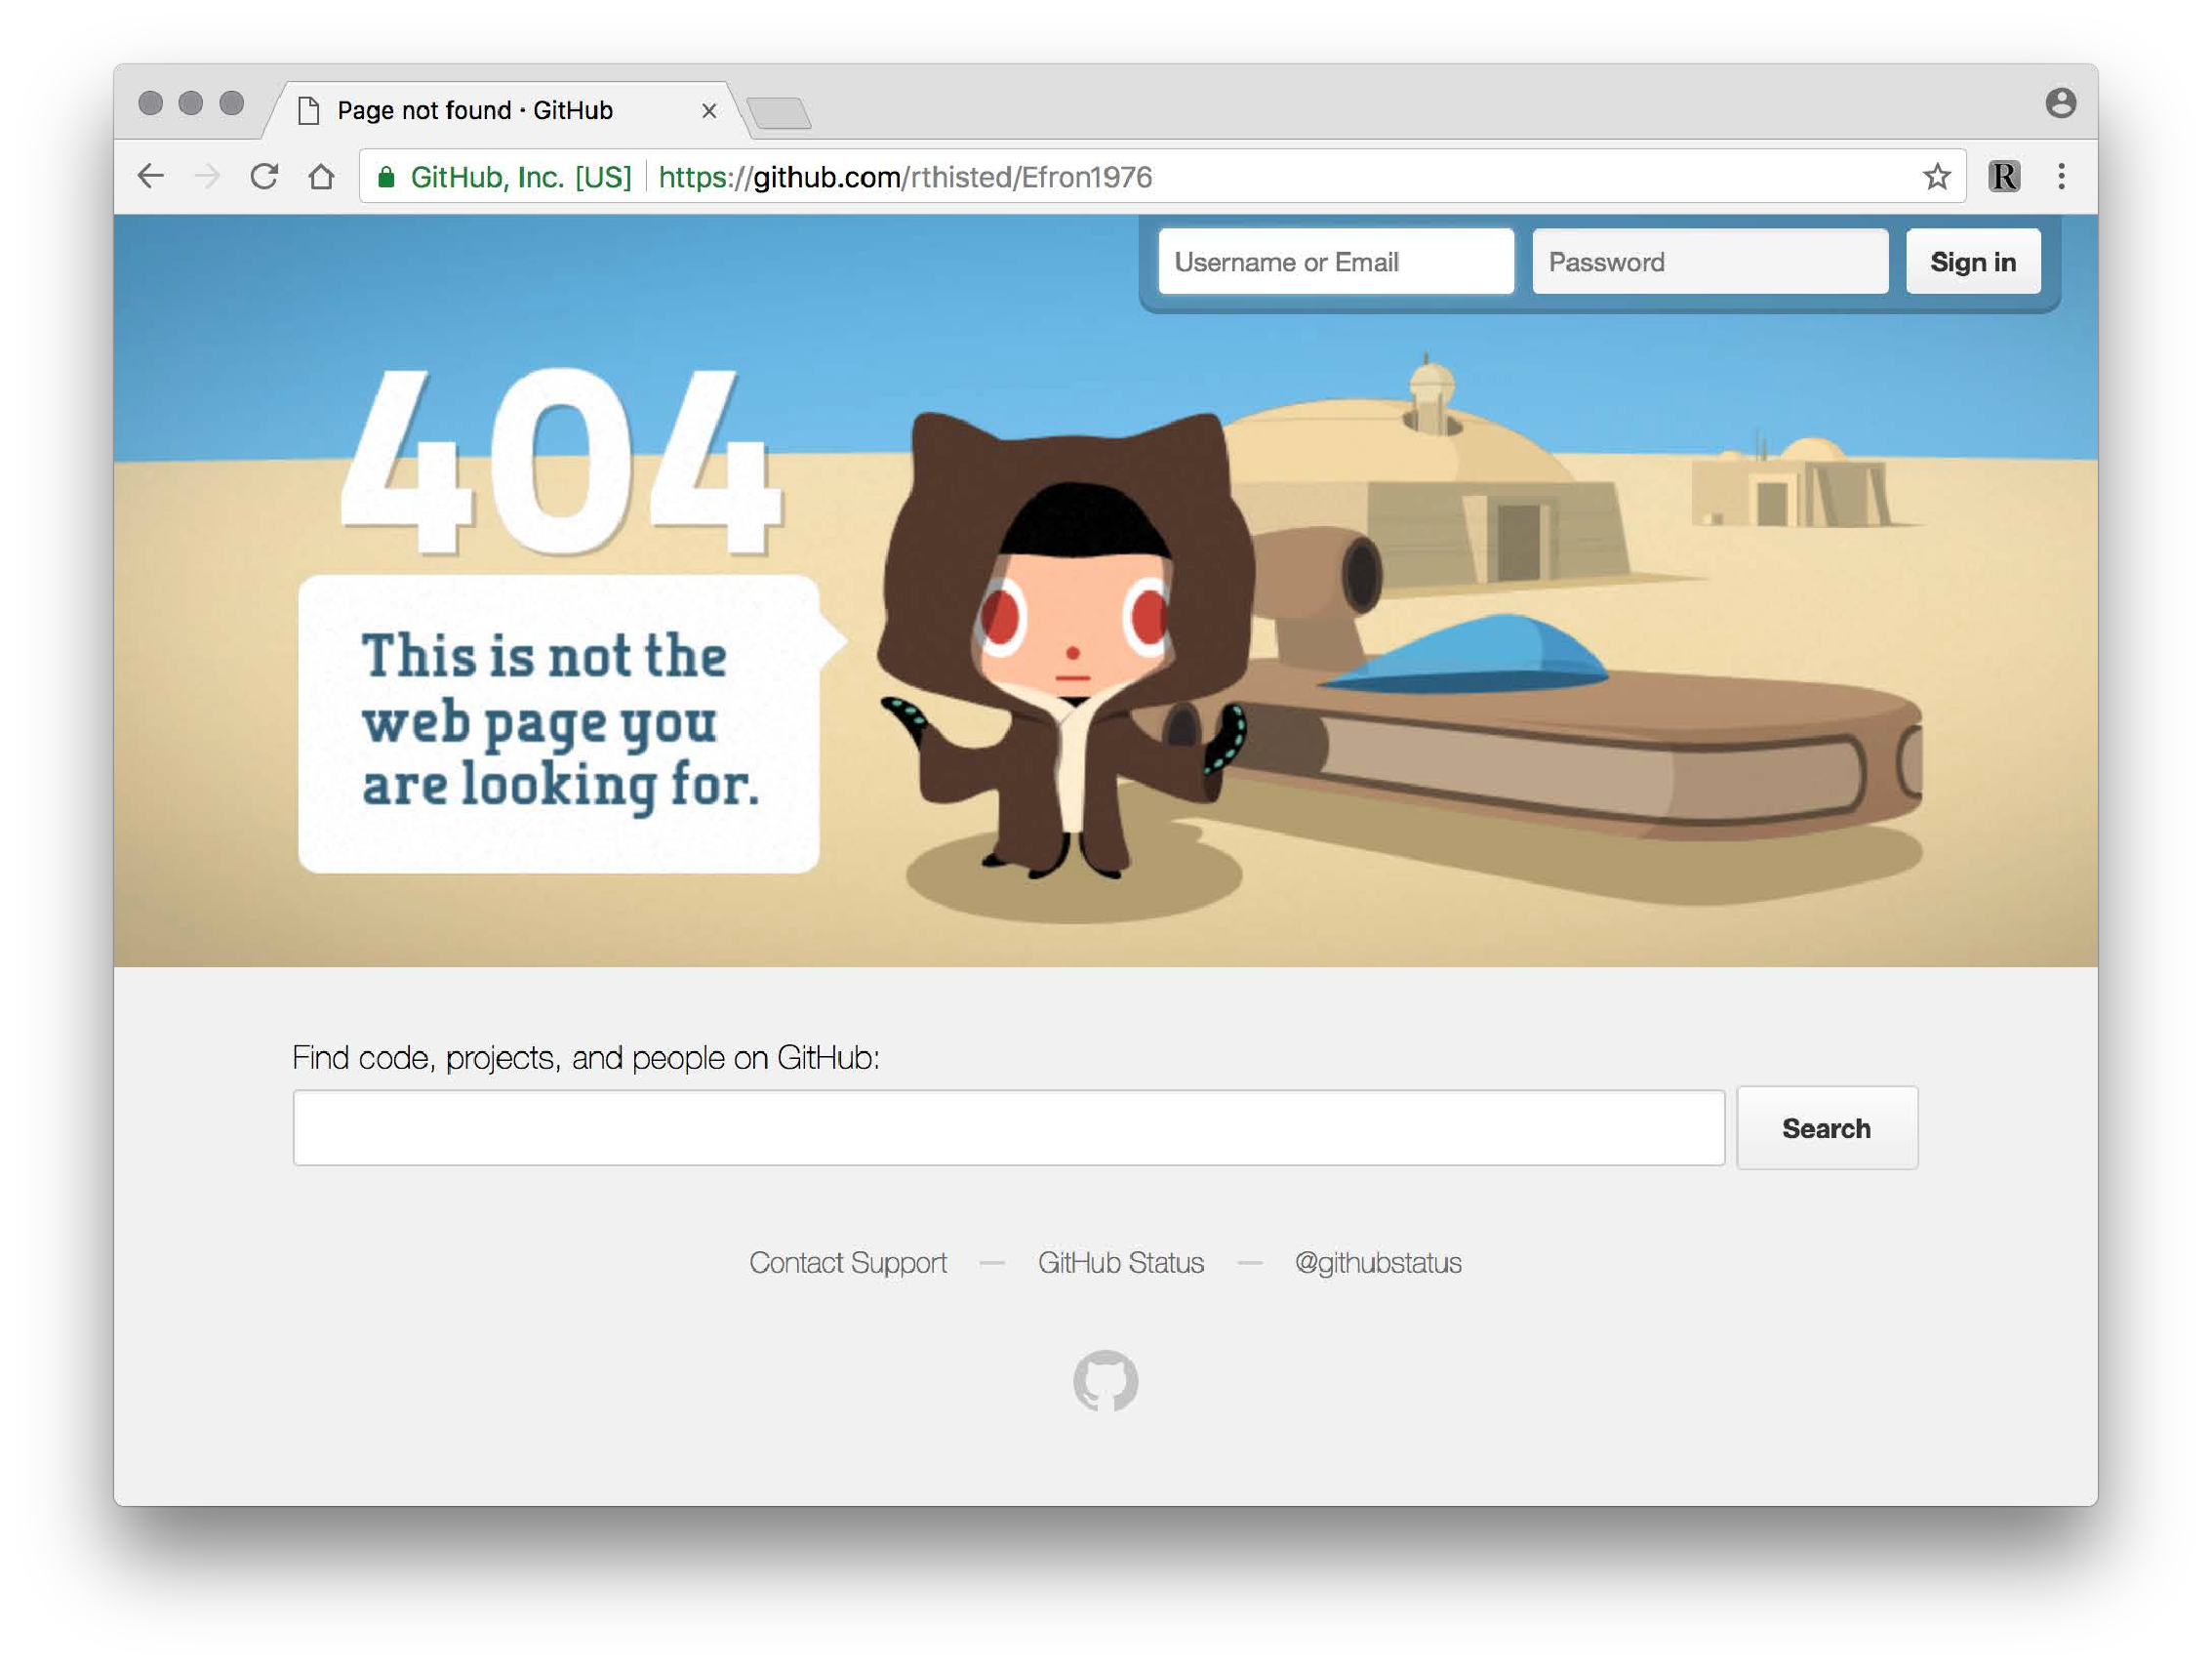
\includegraphics[width=4in]{Photos/github404.pdf}        
    \end{center}  
\end{frame}

	\begin{frame}
    \frametitle{BASIC Program used to calculate Table 3}
    \begin{center}
        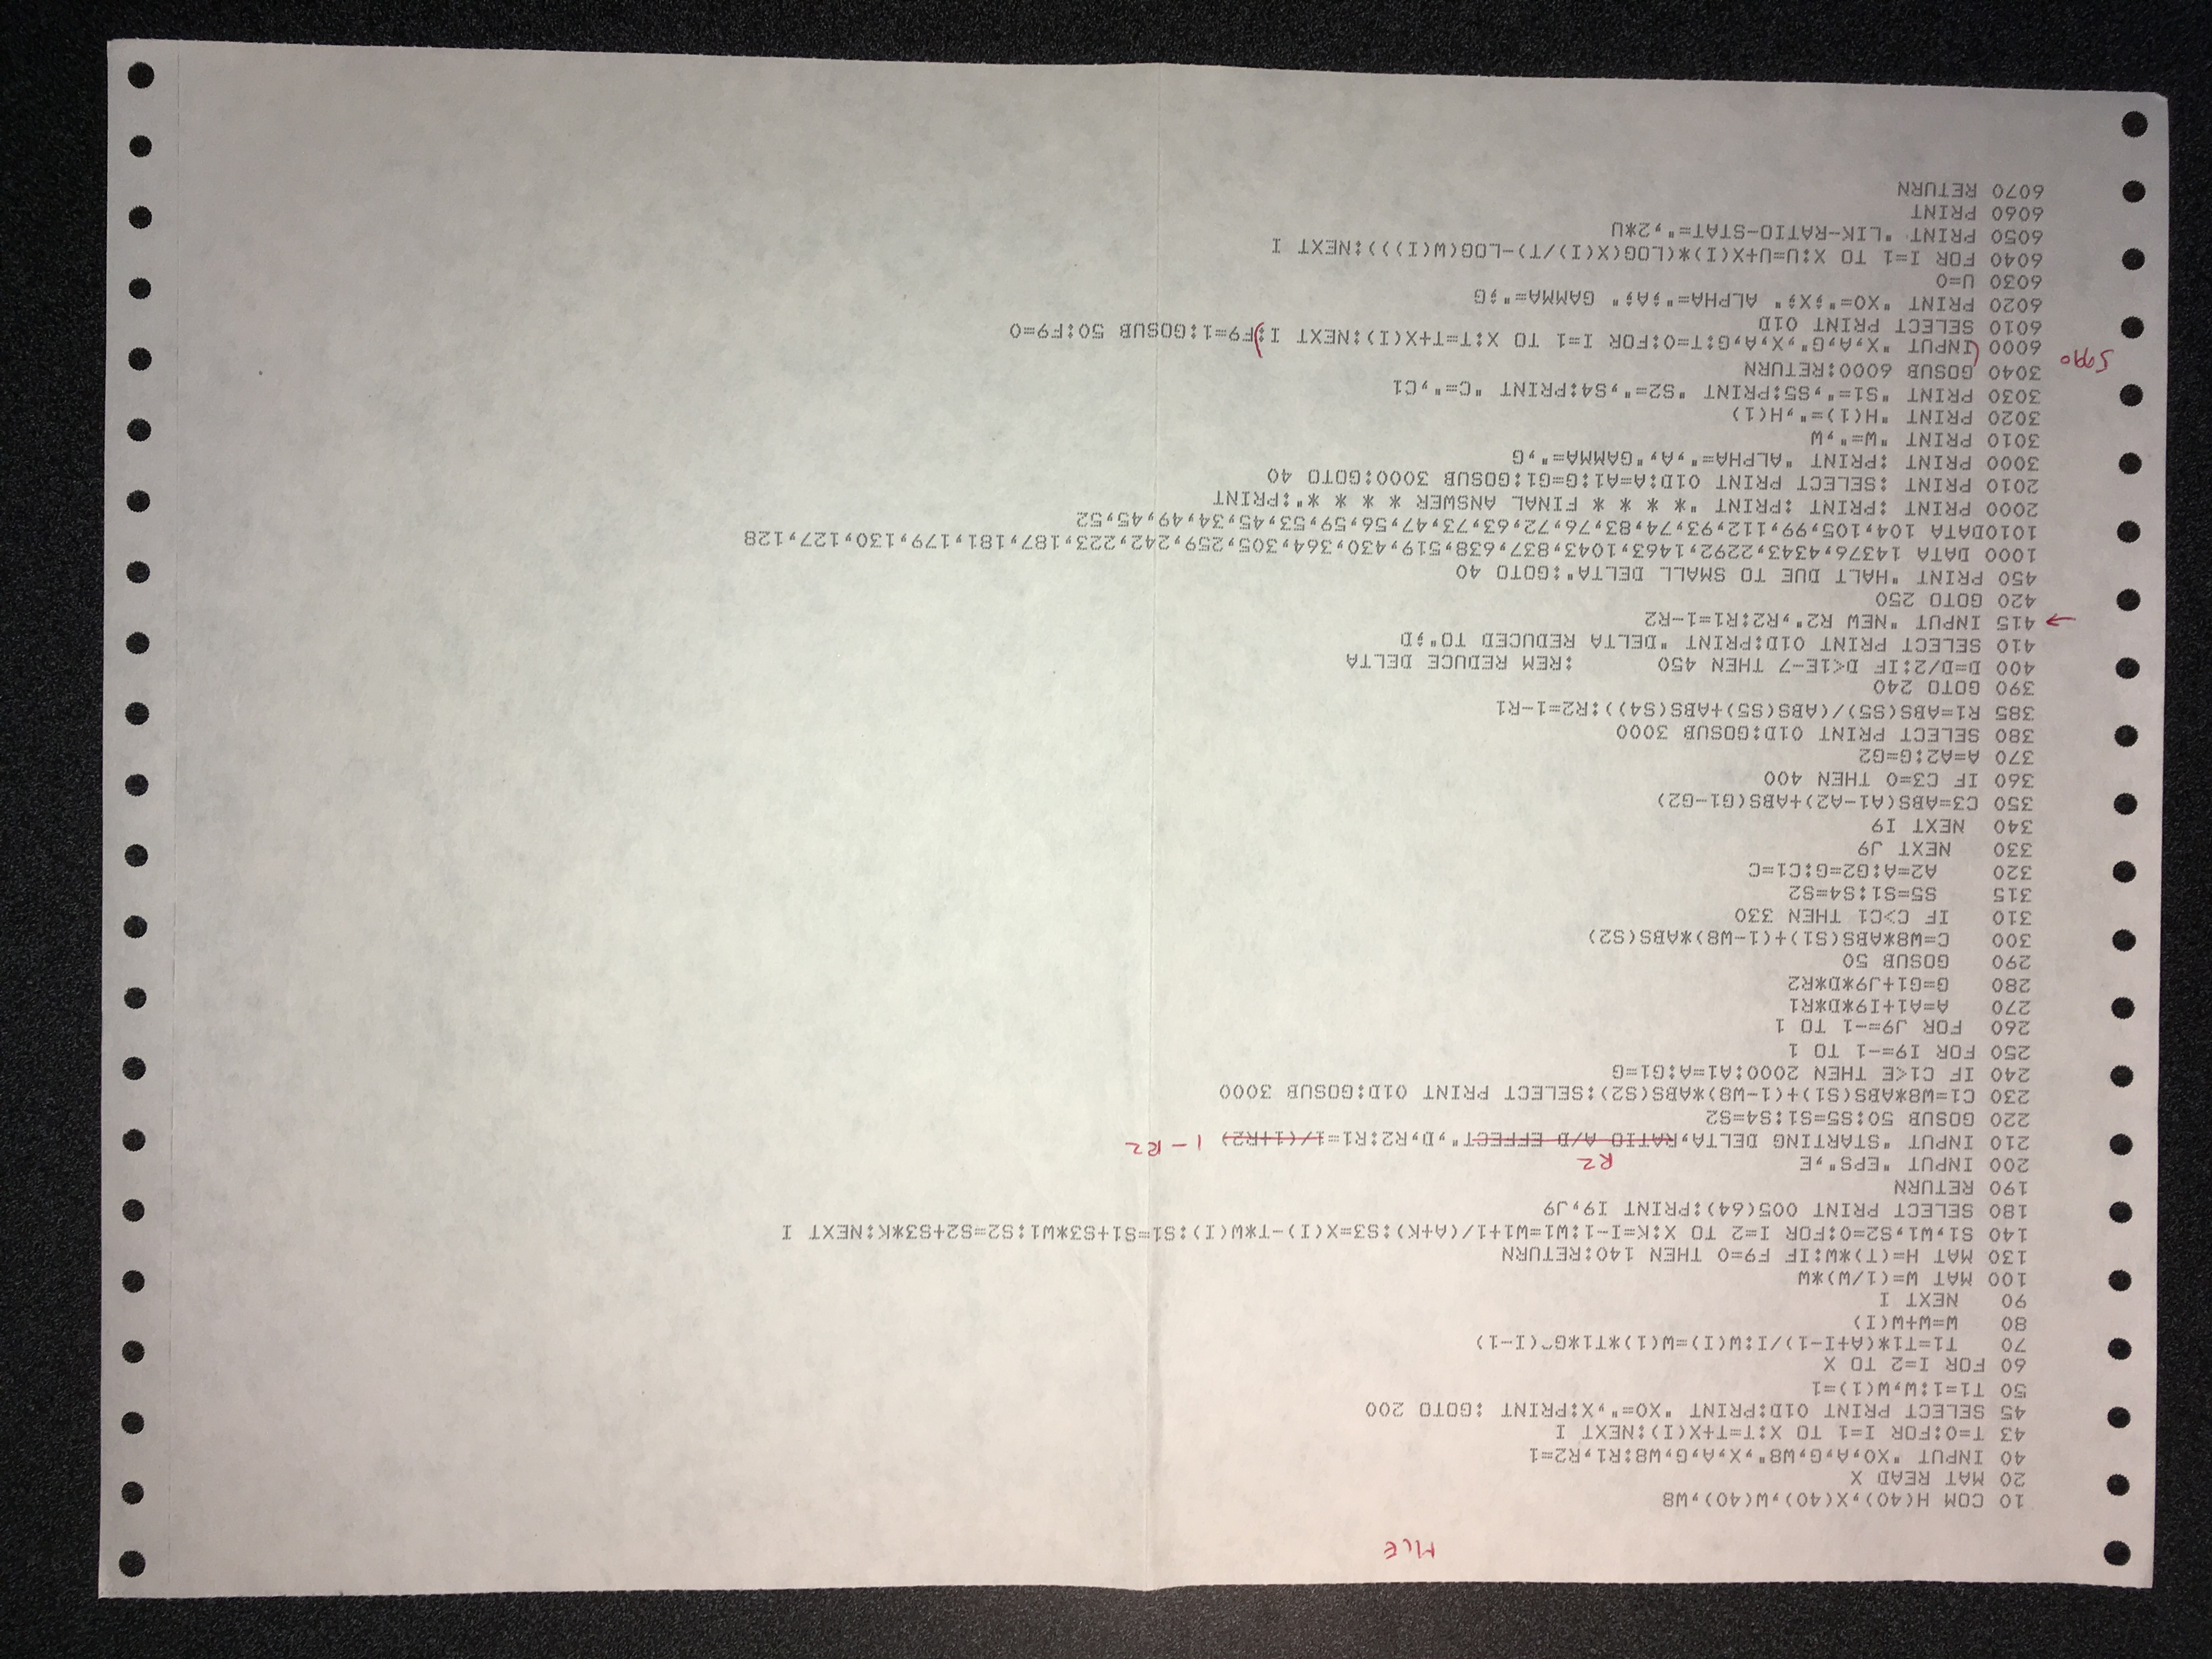
\includegraphics[width=3.5in,angle=180]{Photos/mle-bas-5036.jpg}        
    \end{center}  
\end{frame}

	\begin{frame}[fragile]
    \frametitle{BASIC Program used to calculate Table 3}
		\begin{semiverbatim}\footnotesize
			\input{../Compendium/Programs/mle.bas.txt}
		\end{semiverbatim}
\end{frame}

	\begin{frame}
    \frametitle{The Wang 2200 Computer}
    \begin{center}
        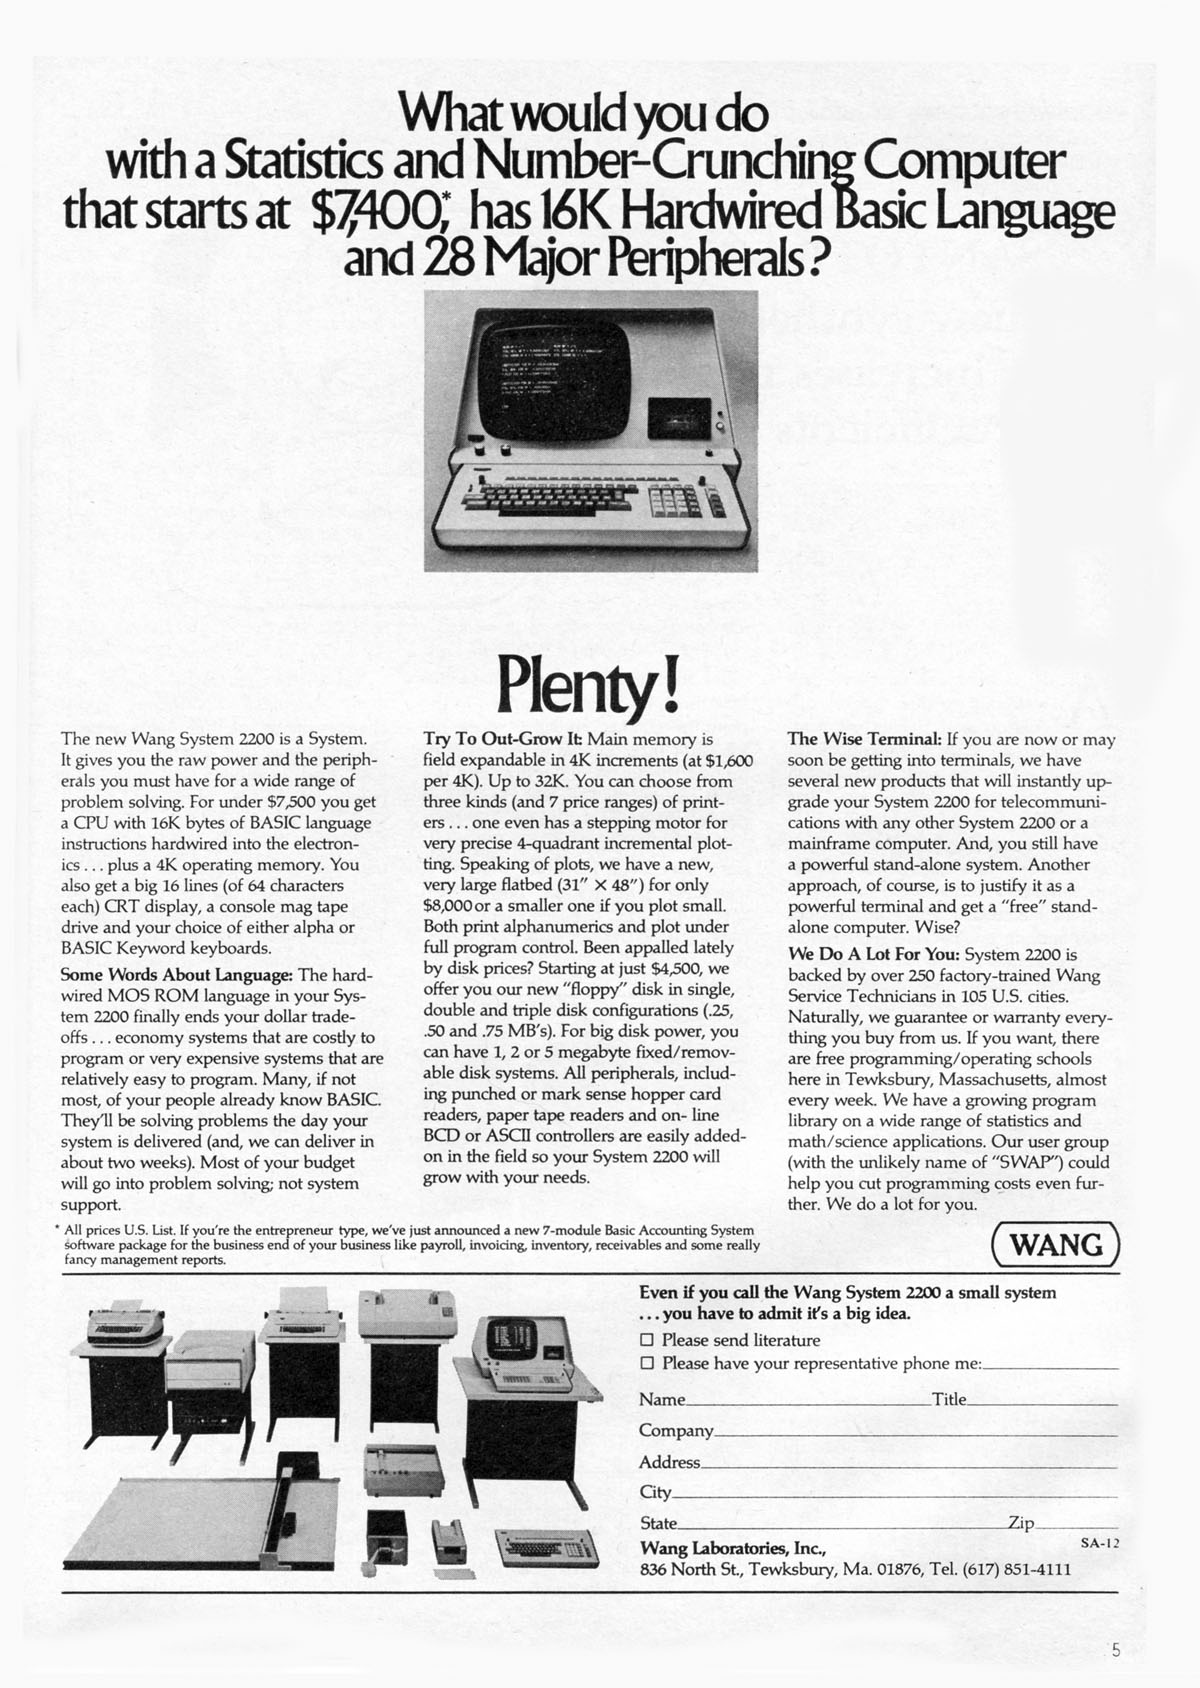
\includegraphics[width=3.5in]{Photos/Wang_System_2200_Computer_1974.jpg}        
    \end{center}  
\end{frame}

	\begin{frame}
    \frametitle{Good News and Bad News}
	\emph{Good news:}  The Wang 2200 has a cult following, and there is an emulator that faithfully reproduces the microcode.
	
	\bigskip
	\emph{More good news:}  The BASIC program actually runs!
	
	\bigskip
	\emph{Bad news:} The ``iterative search'' requires repeated manual inputs, which I didn't write down.
	
	\bigskip
	\emph{More bad news:} I was unable to find values of the inputs that automatically lead to the output parameter values in ET.
	
	\bigskip
	\emph{Some redeeming good news:} The program does reproduce the LR $\chi^2$ values in the paper---and my archived printouts.
\end{frame}

	\begin{frame}
    \frametitle{Archived output for Table~3}
    \begin{center}
		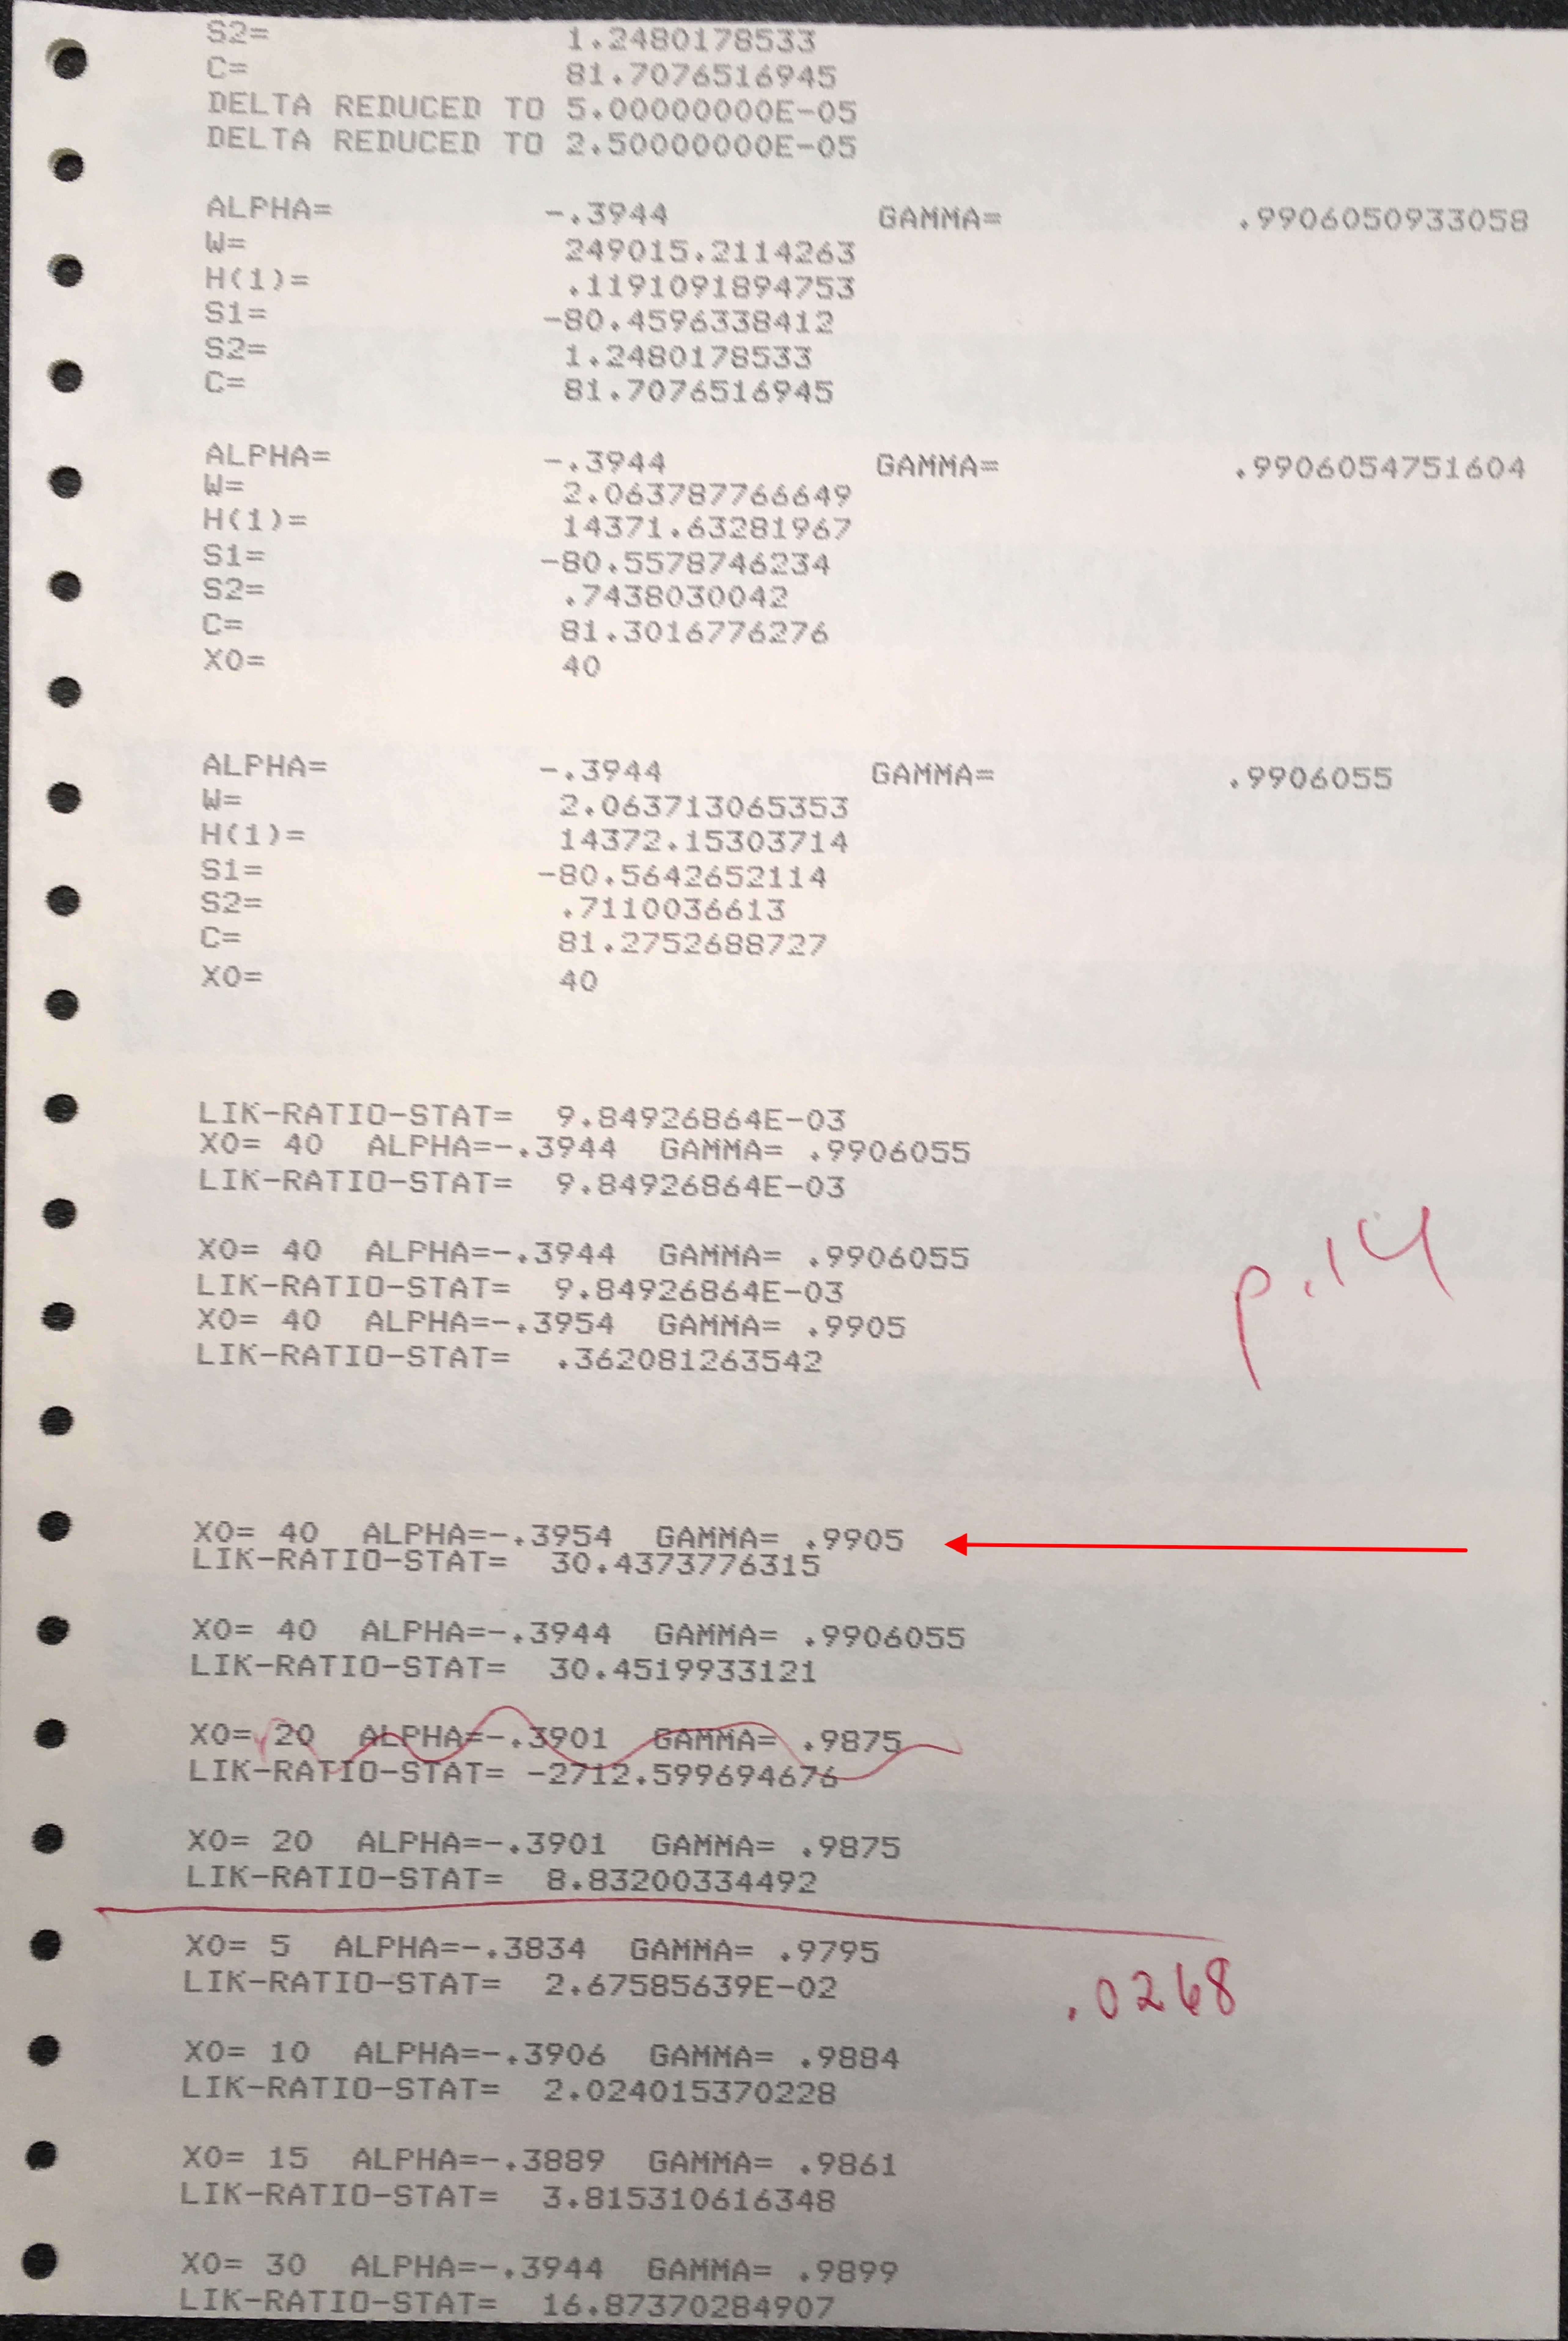
\includegraphics[height=4in]{../Manuscripts/Photos/Table3-output-5037.pdf}        
    \end{center}  
	\medskip
	
	Red arrow points to entry in Table~3 for $x_0=40$, for example.
\end{frame}

	\begin{frame}
    \frametitle{LRT calculations for Table 3}
    \begin{center}
        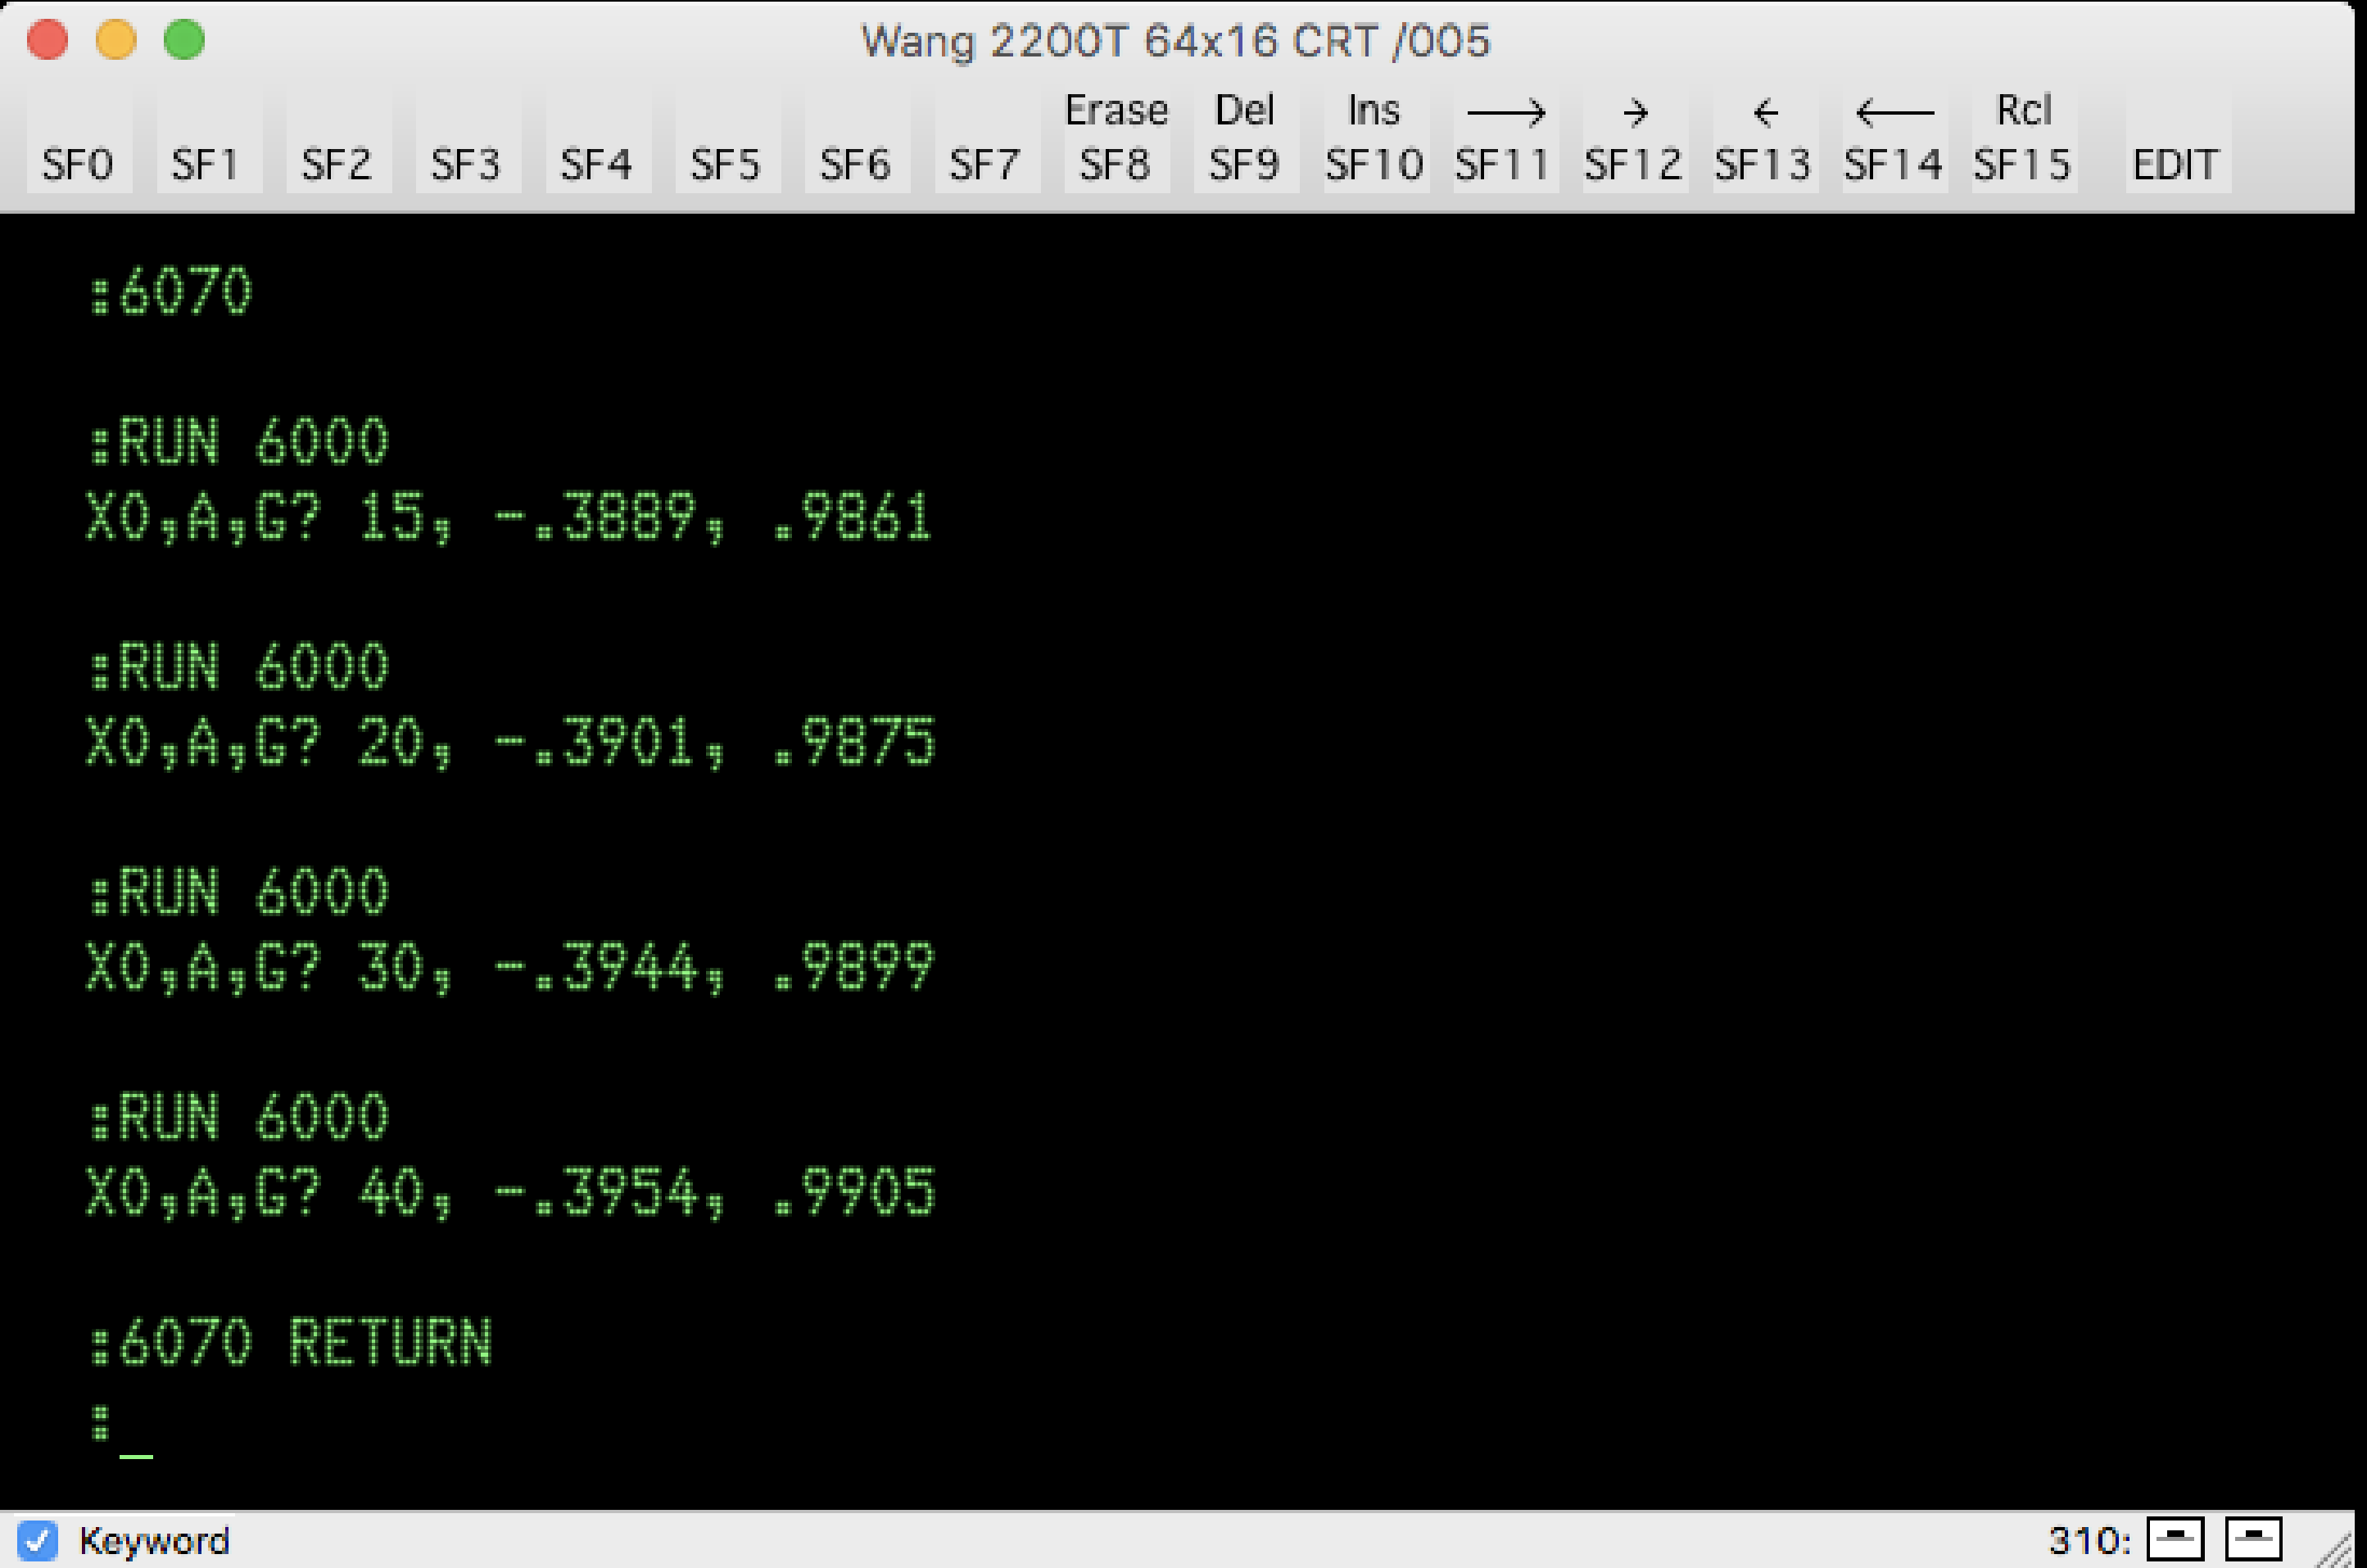
\includegraphics[width=2.25in]{Photos/mle-bas-input-1.pdf}        
        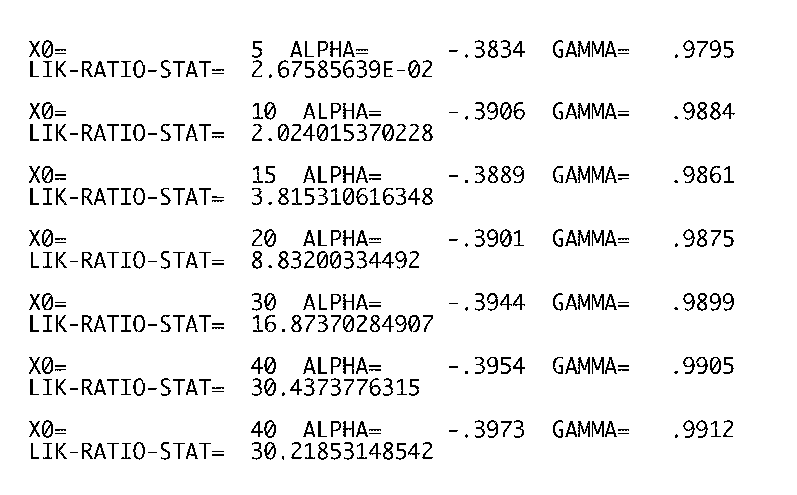
\includegraphics[width=2.5in]{Photos/mle-bas-output-1.pdf}
    \end{center} 
	{\small Excerpt from inputs to the Wang 2200 BASIC program calculating the likelihood-ratio $\chi^2$ statistics (left), and the corresponding outputs (right).  The first six rows of output match both the 1975 computer printout and the entries in Table~3 of ET.  The last row shows the actual MLEs for $x_0=40$; the $\chi^2$ value is somewhat reduced from the value in ET.} 
	 
\end{frame}

\section[Now]{Reproducing Results from ET 1976---Now}
	\begin{frame}
    \frametitle{Advice to a supplicant}
	
	\begin{itemize}
		\item Figure out the likelihood function
		\item Figure out how to maximize while being as lazy as possible
		\begin{itemize}
			\item No hand calculation of partial derivatives of complicated LL fcn
			\item Minimize or eliminate programming
			\item Communicate the method to our student correspondent
		\end{itemize}
		\item Take advantage of widely available software\pause {\color{red} ---Excel!}
		\bigskip
		\item Excel has a built-in black-box maximizer
		\item Excel produces reasonably close to ET Table~3 (but occasional differences in second significant digit)\pause
		\bigskip
		\item Who's right? (Excel not known for outstanding numerics)
		\item Also: \emph{\color{red} Excel spreadsheets are the opposite of reproducible}
	\end{itemize}
\end{frame}

\begin{frame}
	\frametitle{And the answer is\dots.}
	\begin{center}
		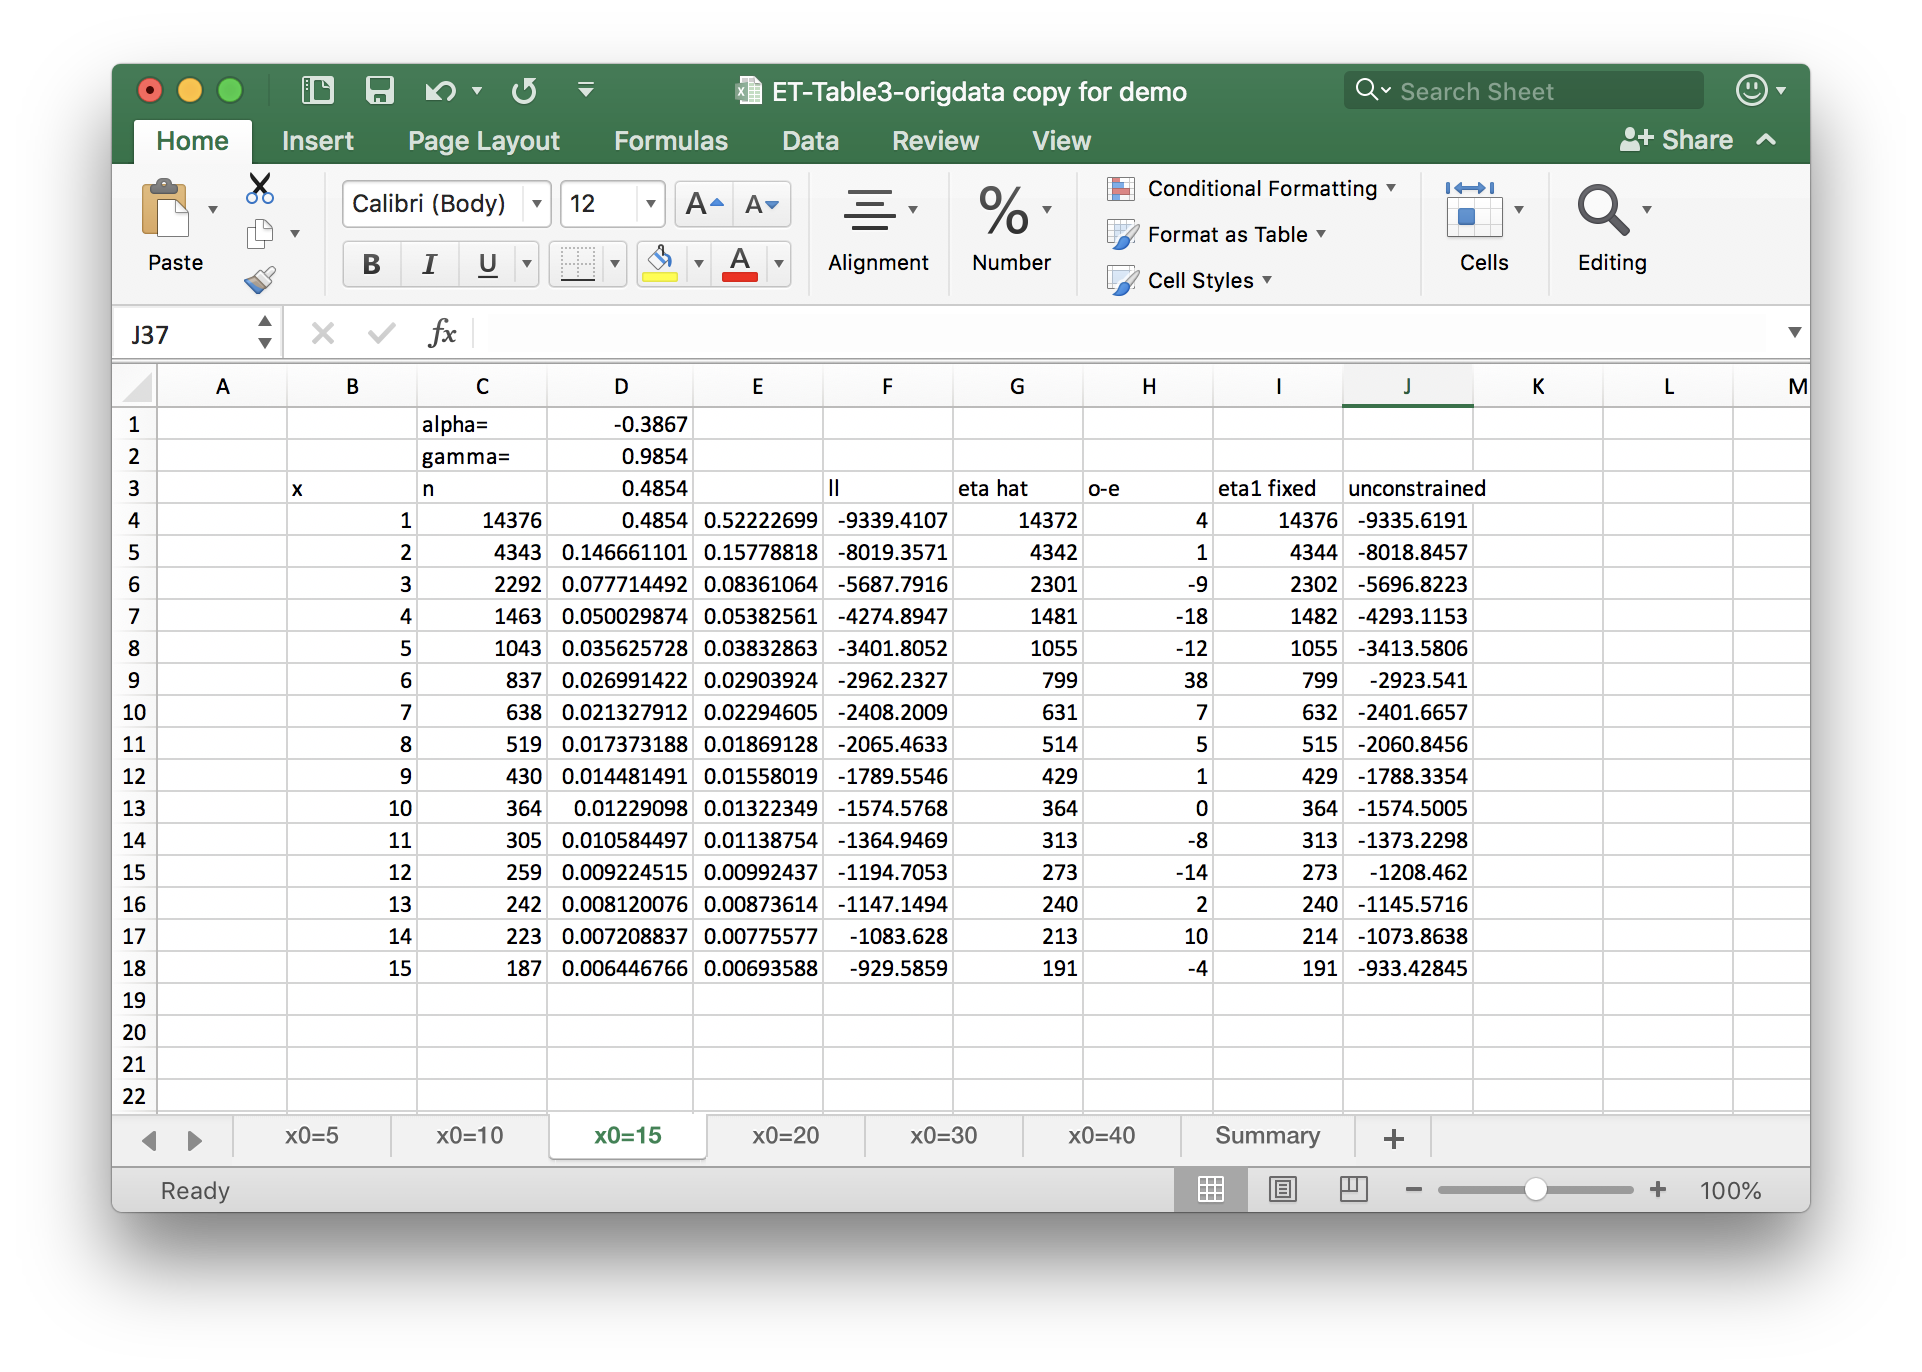
\includegraphics[width=4.5in]{../Manuscripts/Photos/Excel-x0=15.png}
	\end{center}
	
\end{frame}
	\begin{frame}
    \frametitle{A More Satisfactory Approach}
	
	\begin{itemize}
		\item Write scripts for widely-used software
		\item In my case, Stata
		\item Points in favor:
		\begin{itemize}
			\item Outstanding numerics, graphics, data management, scripting
			\item Easy to do general maximum likelihood calculations
			\item Widely used by econometricians, epidemiologists, biostatisticians
			\item Professionally maintained, version controlled execution
			\item (Mostly) open source
			\item Can get standard errors for ML estimates
		\end{itemize}
		\item Points against:
		\begin{itemize}
			\item Proprietary and somewhat expensive
		\end{itemize}
	\end{itemize}
\end{frame}


\begin{frame}
	\frametitle{MLE calculations in Stata}
	\begin{itemize}
		\item Write a script that returns the likelihood given parameters
		\item Write a wrapper the reads the input data, invokes ML program, loops over $x_0$ values
	\end{itemize}
	\bigskip
	\begin{table}
		\centering
		\input{../Manuscripts/StataMLE-Table3-origdata}
		\caption{MLEs using Stata's \texttt{ml} program for maximum likelihood calculation, with the user-written likelihood specification script \texttt{et.do}.}
	\end{table}
\end{frame}

\begin{frame}
	\frametitle{Stata vs Excel}
	\strut
	\bigskip
	
	Stata and Excel agree remarkably well:
	\begin{itemize}
		\item $\hat\alpha$ values agree to~1 unit in 4th decimal place
		\item $\hat\gamma$ values agree to four decimal places
		\item Stata produces very slightly smaller LR $\chi^2$ values
	\end{itemize}
	\bigskip
	
	So, how do the ET 1975 calculations hold up?
	\bigskip
	
\end{frame}

\begin{frame}
	\frametitle{Stata 2018 vs BASIC 1975}
	\strut
	\medskip
	
	Not badly, but certainly not to the precision suggested:
	\bigskip
	\begin{table}
		\centering
\begin{tabular}{rrrrrr}
$x_0$ & $\sum n_x$ & $\hat\alpha$ & $\hat\gamma$ & $\hat\beta$ & $\chi_{x_0-3}^2$\\[3mm]
 5  & 23517  & -0.383\z{5}  &  0.9795 &   47.8\z{0} &   0.027\\
10  & 26305  & -0.390\z{2}  &  0.988\z{3} &   8\z{4.50} &   2.02\z{2}\\
15  & 27521  & -0.38\z{68}  &  0.98\z{54} &   \z{67.44} &   3.\z{752}\\
20  & 28266  & -0.3\z{895}  &  0.987\z{2} &   7\z{7.19} &   8.8\z{22}\\
30  & 29147  & -0.394\z{5}  &  0.9899 &   9\z{8.19} &  16.87\z{3}\\[+3mm]
40  & 29660  & -0.39\z{73}  &  0.99\z{12} &  1\z{12.22} &  30.\z{217}\\
ET-40 & 29660  & -0.3954  &  0.9905 &  104.26 &  30.437\\
\end{tabular}
		\caption{MLEs using Stata \texttt{ml} for maximum likelihood calculation, \z{with differences from ET Table~3}.}
	\end{table}
\end{frame}
	\begin{frame}
	\frametitle{Do these differences matter?}
	\begin{itemize}
		\item The ET parameter estimates at $x_0=40$ are well within $\pm 1\mbox{se}$ of the actual MLEs
		\item The (log) likelihood is pretty flat near the solution, so \dots
		\item Differences in estimates for $\hat\Delta(1)$ are miniscule
	\end{itemize}
	
		\begin{table}
			\centering
			\begin{tabular}{ll}
				& $\hat\Delta(1)$\\[2mm]
				NB-1975 (Wang)     & 11483 \\
				NB-2018 (Stata)    & $11490 \pm 25$ \\[5mm]
				EB-unbiased        & $11430 \pm 178$ \\
				EB-unbiased (corr) & $11486 \pm 178$ \\[5mm]
			\end{tabular}
		\end{table}
\end{frame}
\section[Data]{And what about the data?}
	\begin{frame}
	\frametitle{Data issues}
	
	There are a number of questions related to the \textit{data} that went in to the ET 1975 calculations
	
	\begin{itemize}
		\item We have taken Table~1 from ET as given for this talk, but\dots
		\item The ``simple unbiased estimator'' for $\hat\Delta(1)$ calculated from Table~1 is 11486, not the 11430 reported in the paper!
		\item The only tabulation of the data in my paper archive is a hand-written one that differs from Table~1 in several entries
		\item Going back to Spevack to resolve discrepancies shows that Table~1 is largely correct, with a handful of entries that differ by~1 or~2, but one entry ($n_4$) that is too small by 110.
	\end{itemize}
	
	Fortunately, these discrepancies have little effect on the conclusions of the paper.
\end{frame}
\section[Lessons]{Lessons for the next 40 years}
	\begin{frame}
	\frametitle{Lessons concerning reproducibility}
	
\begin{itemize}
	\item Because {\color{ForestGreen}data sets, programs, computing environment, parameter choices} evolve:
	\begin{itemize}
		\item Need to track and preserve successive versions
		\item Need archived snapshot linking specific data, program versions to specific versions of the manuscript
		\item Good version control tools make this possible
	\end{itemize}
	\item Programs are not enough; need to know what they were trying to do (and why)
	\item Programs that require tuning parameters won't reproduce results unless \textit{the settings used in the published product are preserved.}
	\item Archiving contemporaneous notes can help immensely.
	\item Reproducibility decays with time. (There won't always be a Wang 2200 emulator). Repositories need regular tune-ups.
\end{itemize}	
\end{frame}


\section[Finally]{Concluding remarks}
	\begin{frame}
	\frametitle{And finally, \dots}
	
A public GitHub repository will be available with
		\begin{itemize}
			\item These slides
			\item All supporting programs, scripts, and data
			\item A manuscript (in progress)
			\item Additional supporting materials
		\end{itemize}
		\strut\\
		\texttt{https://github.com/rthisted/EfronAt80}
	\bigskip
	
	Thanks and gratitude to Brad Efron, generous mentor, incredible teacher, incomparable scholar, and friend.
	
	\bigskip
	\begin{quotation}
		 	So on the tip of his subduing tongue\\
		 	All kind of arguments and question deep,\\
		 	All replication prompt and strong,\\
		 	For [our] advantage still did wake and sleep.\\
		 {\qquad\qquad--- \textit{A Lover's Complaint}} %120--123
	\end{quotation}
	
\end{frame}

%	\input{Slides/}


\bibliographystyle{plainnat}
\begin{frame}
    \frametitle{Useful References}\tiny
    \bibliography{../References/Efron80}   
\end{frame}
\nocite{Spevack:1968qd,Efron:1976zs,knuth1984literate,Gani:1976rg,Buckheit:1995hl}

\end{document}

